\documentclass[12pt, oneside]{article}
\usepackage{setup}
\usepackage{import}
\usepackage{graphicx}
\graphicspath{ {./images/} }

% ! Title page settings
\newcommand{\pageauthor}{Yavuz Shahzad}
\newcommand{\pagetitle}{Design of Experiments}
\newcommand{\pagesubtitle}{MATH 558}
\newcommand{\pagedescription}{An introduction to concepts in statistically designed experiments}
\newcommand{\pagesemester}{Winter 2025 }
\newcommand{\pageprofessor}{Prof. Alia Sajjad}

\begin{document}


\thetitle

\setstretch{1.3}
{\scshape\tableofcontents}\newpage


\pagestyle{mypage}

\newgeometry{margin=0.3in, top=0.4in, bottom=0.5in, marginparwidth=1.4in, marginparsep=0.3in}
\parskip=0.6em


% creates references for every section and subsection
\let\origsection=\section
\let\origsubsection=\subsection

\renewcommand\section[1]{\origsection{#1}\label{\thesection}}
\renewcommand\subsection[1]{\origsubsection{#1}\label{\thesubsection}}


% ! import parts here
\foreach \i in {00, 01, 02, 03, 04, 05, 06, 07, 08, 09, 10, ..., 99} {%
    \edef\FileName{parts/\i.tex}%
    \IfFileExists{\FileName}{%
      \input{\FileName}
      \begin{center}
        \hrule
        \hfill\textit{\tiny{$\hookrightarrow\,$Lecture \i; Last Updated: \input{|"date -r  "\FileName}}}
      \end{center}
    }
  }

\newpage
% \setstretch{1.5}
% \pagestyle{mypage}
% \listoftheorems[ignore={remark}, title={\section{List of Theorems}}, swapnumber]

This course follows the text \textit{Design of Comparative 
Experiments by R. A. Bailey (Cambridge Series in Statistical and Probabilistic Mathematics.}

\section{Chapter 1. Forward Look}

\subsection{Stages in a Statistically Designed Experiment}
\subsubsection{Consultation}

Ideally, the consultation process should start well before data collection begins. However, the statistician usually does not have control of this. 

If contacted close to the time when the experiment needs to start, one should ask enough questions to get a clear idea of the experiment. Importantly, get an idea of the purpose, the resources at the researchers' disposal, the timeline, etc. Ask these questions carefully because researchers may not be aware of what information is necessary to design an experiment.

\textbf{Discussion of Example 1.1 (Ladybirds) in Bailey (pg. 2)}

\textbf{Ex 1.1:} A famous company (which I shall not name) had designed an
experiment to compare a new pesticide which they had developed, a standard pesticide, and
‘no treatment’. They wanted to convince the regulatory authority (the Ministry of Agriculture,
Fisheries and Foods) that their new pesticide was effective but did not harm ladybirds.
I investigated the data from the experiment, and noticed that they had divided a field into
three areas, applied one pesticide (or nothing) to each area, and made measurements on three
samples from each area. I asked the people who had designed it what the design was. \textbf{They said that it was completely randomized} (see Chapter 2). I said that I could see that it was not
completely randomized, because all the samples for each pesticide came from the same area
of the field. They replied that it must be completely randomized because there were no blocks
(see Chapter 4) and it was not a Latin square (see Chapter 6). In defense of their argument
they quoted a respectable textbook which gives only these three designs.

This anecdote goes to show that misconceptions about experimental design are prevalent in the scientific community. A statistician should keep this in mind when consulting for experts in other fields. 

\subsubsection{Data Collection}

The (statistical) design of experiments (DOE) is step by step process for planning experiments so that the data obtained from the experiment can be analyzed to yield  conclusions. A good experimental design is based on clearly defining the objectives of the experiment and using the available resources in effective manner to draw the required information.

\textbf{Important tips for data collection:}
When collecting data, create a row for \textbf{each observational unit} and a column for each \textbf{treatment.} Include a few extra columns to record any additional variables that might emerge during the observation. If the data is collected by the researcher, instruct them to retain the data in its raw form to minimize copying or cleaning errors. 

\subsubsection{Data Scrutiny}

After the experiment is done, the data sheets or data files should be sent to the statistician
for analysis. Look over these as soon as possible for obvious anomalies, outliers or evidence
of bad practice.

\textbf{Example 1.3 (Leafstripe)} In an experiment on leafstripe disease in barley, one measurement
was apparently the percentage of disease on each plot. A preliminary graph of the data showed
one outlier far away from the rest of the data. I asked to see the data for the outlying plot, and
was given a collection of pieces of paper like those shown in Figure 1.1. It transpired that the
agronomist had taken a random sample of ten quadrats in each plot, had inspected 100 tillers
(sideshoots) in each quadrat to see how many were infected, and averaged the ten numbers.
Only the average was recorded in the ‘official’ data. For the outlying plot the agronomist
rightly thought that he did not need a calculator to add nine zeros to one nonzero number, but
he did forget to divide the total by 10. Once I had corrected the average value for this plot, it
fell into line with the rest of the data.

Also see Examples 1.4-6 in Bailey's text.

\subsubsection{Data Analysis}

Your data analysis plan should be thought of before you design your experiment. \textbf{The information you want to draw from your data affects the way you collect your data.} 

\subsection{The Ideal and the Reality}

\subsubsection{Purpose of the Experiment}

In designing an effective experiment, one needs to understand the purpose of the experiment. For example, what are the treatments that need to be compared? What is the research question being asked? What is the population to which the results will be extended?

\subsubsection{Replication}

Replication refers to the number of times each experimental treatment is tested (not replication of an experiment by other researchers). Specifically, \textbf{it is the repeating of an experimental condition to different experimental units.} Each repetition is an independent observation under the same conditions (never a re-measurement of the same experimental unit).

Replication measures variability in the experiment, improves the precision of the results (will typically reduce the statistic $\sqrt{\frac{s^{2}}{n}}$ and thereby tightens the confidence interval), and ensures the results are reliable and generalizable. 



Recall that the formula for the variance of the mean of n observations is 
$var (\overline{X}) = \frac{\sigma^{2}}{n}.$ Increasing the replication then increases n and thereby 
typically decreases the variance. The increase in replication may, however, increase the value of $\sigma^{2}$ thereby 
increasing the variance if it outweighs the increase in n.

Increased replication typically increases power, as it raises the number of residual degrees of freedom: certain 
families of distribution (such as the t-distribution) have slimmer tails with more degrees of freedom. 

\subsubsection{False Replication}

False replication occurs when repeated measurements are taken on the same experimental unit and are treated as independent 
replications. For example, measuring the same plant multiple times and treating each measurement as an independent 
replication, observing a slight difference due to measurement error each time. As a consequence, it overestimates 
the amount of data available, leads to incorrect conclusions about treatment effects, and compromises the reliability of 
the experiment. 

\subsubsection{Defining Terms}

We define the following important terms:

\textbf{Definition: } An \textit{experimental unit} is the smallest unit to which a treatment can be applied. Each experimental unit is inherently different from the other, even when the same treatments are applied to them; the inherent differences between them are spoken to by the experimental error. 

\textbf{Definition:} A \textbf{treatment} is the entire description of what can be applied to an experimental unit.

\textbf{Definition: } An \textit{observational unit} is the smallest unit on which a response can be measured. 

\subsubsection{Local Control}

Another way to reduce $var (\overline{X}) = \frac{\sigma^{2}}{n}.$ is to reduce the variance (a.k.a the experimental error) $\sigma^{2}$ itself. One way of reducing the experimental error is to \textbf{group experimental units into homogeneous (alike) blocks}; this grouping is called \textit{\textbf{blocking}} (discussed further in Chapter 4). 

If done well, blocking lowers the variance $\sigma^{2}$ by removing some sources of variability from treatment contrasts. If each block is representative rather than homogeneous then blocking has the opposite effect. Because blocking generally reduces variance, it typically increases power. However, in the event of small sample sizes, the reduction in $\sigma^{2}$ may be counteracted by the reduction in degrees of freedom, thereby lowering power. 

Additionally, blocking increases the complexity of the design, which makes the statistical analysis and interpretation of the results more difficult.

\subsubsection{Introductory Example: Rye Grass}

We will often refer to the following example: (Bailey pg. 7-8)

\textbf{Example 1.7 (Rye-grass)} An experiment was conducted to compare three different cultivars
of rye-grass in combination with four quantities of nitrogen fertilizer. Two responses were
measured: one was the total weight of dry matter harvested from each plot, and the other was
the percentage of water-soluble carbohydrate in the crop.
The three cultivars of rye-grass were called Cropper, Melle and Melba. The four amounts of fertilizer were 0 kg/ha, 80 kg/ha, 160 kg/ha and 240 kg/ha.

The experimental area consisted of two fields, each divided into three strips of land. Each
strip consisted of four plots. Cultivars were sown on whole strips because it is not practicable to sow them in small
areas unless sowing is done by hand. In contrast, it is perfectly feasible to apply fertilizers to
smaller areas of land, such as the plots. The layout for the experiment is shown in Figure 1.2.
Notice the pattern. Each amount of nitrogen is applied to one plot per strip, and each
cultivar is applied to one strip per field. This pattern is the combinatorial design.
Notice the lack of pattern. There is no systematic order in the allocation of cultivars to
strips in each field, nor any systematic order in the allocation of amounts of nitrogen to plots
in each strip. This lack of pattern is the randomization.

\section{Lecture 6}

\subsection{ANOVA Assumptions}

Previously, we used ANOVA to test the difference between treatment means or whether the treatment effects are non-zero. Also recall that we stated some assumptions that the error terms are required to follow for the validity of the analysis. These assumptions state that the errors are independent and identically distributed with mean 0 and variance $\sigma^{2}$.

Practically speaking, we can apply a Shapiro-Wilkes test to each the normality of the residuals of each treatment mean. Another standard way to test the residuals is to plot a graph. We define the residual 
\[e_{iw} = y_{iw} - \hat{y}_{iw}\] where $\hat{y}_{iw} = \hat{\mu} + \hat{\tau}_{i} = \hat{\mu} + \hat{\mu}_{i} - \hat{\mu} = \bar{y}_{i}$.

In order to test the assumption of constant variance, we will graph (in a scatter plot) the model residuals against factor levels. This scatter plot can reveal the differences in the variability across different levels. By default, R uses standardized residuals.

An example of an issue in the variability might be trumpetting, where the variability in the residuals increases as the treatment mean increases. This is visible in the Residuals vs Fitted plot. 

A statistical test for constant variance is Bartlett's test.

\subsection{Comparison among $\tau_{i}$'s}
In the previous lecture, we covered the estimation of the effect of a treatment $i$, $\hat{\tau}_{i}$, and discussed 
how the effect of any treatment is estimated by taking the mean of the observations related to that particular treatment 
and the overall mean $(\mu_{i} - \mu)$. We saw that a linear model can speak to both these differences in treatment means 
and their associated standard errors. However, what if we concern ourselves with estimating linear combinations of taus, 
such as $\tau_{1} - \tau_{2}$ or $\frac{\tau_{1} + \tau_{2}}{2} + \frac{tau_{3} + \tau_{4}}{2}$. \newline


\textbf{Def: (Contrast)} A linear combination of $\tau_{i}$'s \[l_{m} = a_{m_{k}}\tau_{1} + \cdots + a_{m_{k}} \tau_{k}\]is called a contrast if $a_{m_1} + \cdots + a_{m_{k}} = 0$. 

For example, the combinations $\frac{\tau_{1} + \tau_{2}}{2} + \frac{tau_{3} + \tau_{4}}{2}$ and $\tau_{1} - \tau_{2}$ are contrasts. 

\section{Lecture 7}

\subsection{Orthogonality}

Orthogonality is important in DOE because it corresponds to zero correlation among the estimators of interest. Experimental analysis of an orthogonal design is usually straightforward because you can estimate each main effect and interaction independently. Therefore, any procedures in the analysis of experimental designs are based on the decomposition of data vectors into orthogonal components. 

\textbf{Def: (Orthogonal Design)} Orthogonal designs are experiments where the treatment factors are arranged in such a way that their effects can be independently estimated. This independence ensures no confounding between factors and allows for straightforward interpretation of results. 

Recall that we represented the set of all experimental units as $\Omega$. We can associate an N-dimensional vector space $V$ with $\Omega$. This space $V$ has vectors of the form $v = (v_{1}, \cdots, v_{N})$. The treatment subspace of $V$ is the space generated by the vectors which are constant on each treatment. In other words, $v \in V_{T}$ if the components $v_{(i)}$ are equal for $i$ corresponding to the same treatment. We will denote the treatment subspace by $V_{T}$. See a visualization below: \newline

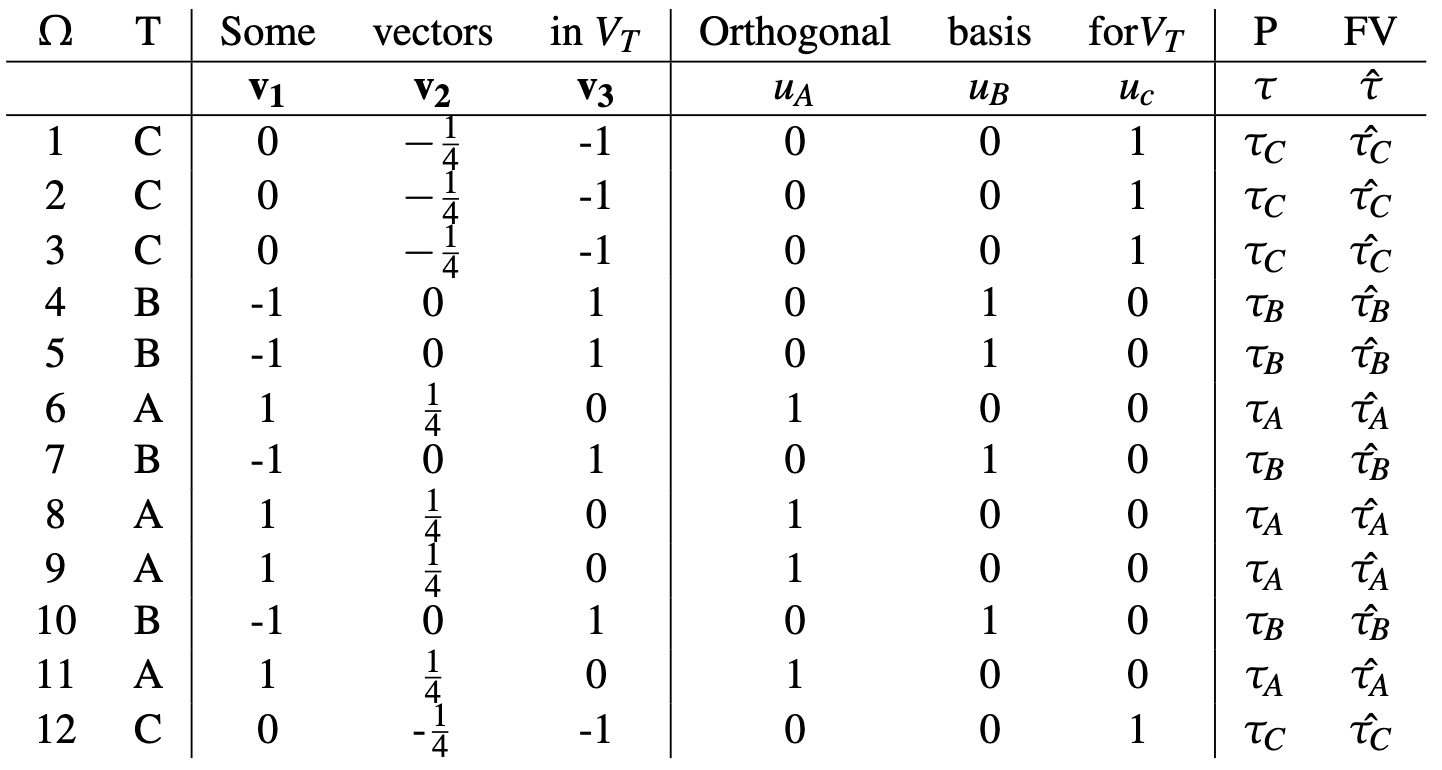
\includegraphics[width = 18cm]{images/TreatmentSubspace.png}

A vector $v \in V$ is a treatment vector if $v \in V_{T}$. You can see that the given $v_{1}$ is a treatment vector because for each entry corresponding to treatment C, $v_{1} = 0$. Likewise for treatments A and B, $v_{1} = -1$ and $v_{1} = 1$, respectively. In fact, vector $v_{1}$ represents the contrast $\tau_{A} - \tau_{B}$.

A vector space itself, $V_{T}$ has an orthogonal basis. These are given in the figure above,and their construction is as to be expected. In our three-treatment example, $V_{T}$ is a three dimensional subspace, and each of the orthogonal basis vectors corresponds to some treatment. Where the experimental unit is in the associated treatment, the basis vector takes the value of 1, and takes the value of 0 otherwise. 

For each treatment $i$, let $u_{i}$ be the vector whose value on the plot $\omega$ is 1 if plot $\omega$ gets the treatment $i$ and 0 otherwise. Then the orthonormal basis is composed of all $u_{i}$ for $i \in T$. Note that every vector in $V_{T}$ is a unique combination of $u_{i}$.

It follows that (using notation from linear algebra) $u_{i}^{T}u_{j} = 0$ when $i \neq j$, and $u_{i}^{T}u_{i} = r_{i}$ where $r_{i}$is the replication of treatment $i$.

\subsection{Orthogonal Projection}

If $W$ is a subspace of $V$then the orthogonal complement of $W$ is denoted by $W^{\perp} := \{v \in V : v \perp w \;\forall w \in W \}$. \newline

\textbf{Theorem:} Let $W$ be a subspace of $V$. Then the following holds:

\begin{enumerate}
    \item[i.] $W^{\perp}$ is also a subspace of $V$.
    \item[ii.] $(W^{\perp})^{\perp} = W$.
    \item[iii.] $ \dim (W^{\perp}) = \dim(V) - \dim(W)$.
    \item[iv.] $V$ is the direct sum $W \oplus W^{\perp}$.
    
\end{enumerate}

Item iv means that given any vector $v \in V$, there are unique vectors $x \in W, \; z \in W^{\perp}$ such that $v \ x + z$. We call $x$ the orthogonal projection of $v$ onto $W$ and denote it by $x = P_{W}(v)$. Since orthogonal projection is a linear transformation, it can also be represented by an N x N matrix.

\begin{enumerate}
\item[v.] The orthogonal projection of a vector $v \in V$,denoted by $P^{\perp}_{W}(v)$, is given by $P^{\perp}_{W}(v) = z = v - x$.

\item[vi.] For a fixed vector $v \in V$ and a vector $w \in W$, the sum of squares of the differences is: \[\sum_{w \in W} (v - w)^{2} = ||v - w||^{2}\]

This sum is minimized when $w = P_{W}v$.

\item[vii.] If $\{ u_{1}, \cdots , u_{n}\}$ is an orthogonal basis for W, then the projection of $v$ onto $W$ is $P_{W}v = \frac{v^{T}u_{1}}{||u_{1}||^{2}} u_{1} + \cdots + \frac{v^{T}u_{n}}{||u_{n}||^{2}} u_{n}$.

\end{enumerate}

Let $V = \mathbb{R}^{3}$ spanned by $e_{1}, e_{2}, e_{3}$. Let $W \subseteq V$, where $W$ is spanned by $e_{1}, e_{2}$.  The orthogonal projection of $v$ onto $W$ is $\frac{v^{T}e_{1}}{||e_{1}||^{2}} e_{1} +  \frac{v^{T}e_{2}}{||e_{2}||^{2}} e_{2} = \; (v_{1}, v_{2}, 0)^{T}$.

The projection can also be represented as a matrix since 

\begin{math}
P_{W}v = \frac{u_{1}v^{T}}{||u_{1}||^{2}}u_{1}  + \cdots + \frac{u_{n}v^{T} }{||u_{n}||^{2}}u_{n}  \in \mathbb{R}^{N \times N}
\end{math}

Note that the matrix $P_{W}$ is symmetric ($P^{T}_{W} = P_{W}$) and idempotent ($(P_{W})^{2} = P_{W}$), and that the trace of $P_{W}$ is equal to the dimension of $W$.


\section{Lecture 8}

Two contrasts are said to be orthogonal if the sum of products of their corresponding coefficients is zero. That is, for two contrasts
$l_{m} = a_{m_{1}}\tau_{1} + a_{m_{2}}\tau_{2} + \cdots + a_{m_{t}}$ and 
$l_{n} = a_{n_{1}}\tau_{1} + a_{n_{2}}\tau_{2} + \cdots + a_{n_{t}}$ are orthogonal iff 
$a_{m_{1}} a_{n_{1}} + \cdots + a_{m_{t}} a_{n_{t}} = 0$.

Orthogonality in the contrasts ensures that the contrasts are independently distributed. 

The vector $\tau$ in the previous table is a vector of unknown parameters. We also know that $\tau \in V_{T}$. 
Therefore it can be written as a linear combination of the vectors in the orthogonal basis of $V_{T}$. That is,
$\tau = \tau_{A} u_{A} + \tau_{B} u_{B} + \tau_{C} u_{c}$.

\textbf{Theorem: } Consider the linear model
\begin{equation}
Y = \tau_{1} u_{1} + \cdots + \tau_{t} u_{t} + \epsilon
\end{equation}

where $\mathbb{E}(\epsilon) = 0, \; Cov(\epsilon) = \sigma^{2}I$. Also, let $W$ be a subspace of $V$. Then the following hold:

\begin{itemize}

  \item[i.] $\mathbb{E} (P_{W} Y) = P_{W} (\mathbb{E}(Y)) = P_{W}\tau$.
  \item[ii. ] $\mathbb{E}(||P_{W} (Y)||^{2}) = ||P_{W} \tau||^{2} = \dim (W) \sigma^{2}$

\end{itemize}

\textbf{Proof: }

$Y = \tau_{1} u_{1} + \cdots + \tau_{t} u_{t} + \epsilon$ with $\mathbb{E} (\epsilon) = 0$. This implies, by the linearity
of expectation that $\mathbb{E} (Y) = \tau \in V_{T}$ and $Cov(Y) = \sigma^{2}I$. Hence, it follows that 
$\mathbb{E} (P_{W}Y) = P_{W} \mathbb{E}(Y) = P_{W} \tau$.

\section{Lecture 9}

\textbf{Proof cont. }



\end{document}
